\chapter{Validation \& Testing}

\section{Cutting Tests}
To validate the line cutter, a series of cutting tests were performed. 

\begin{figure}[h!]
    \centering
	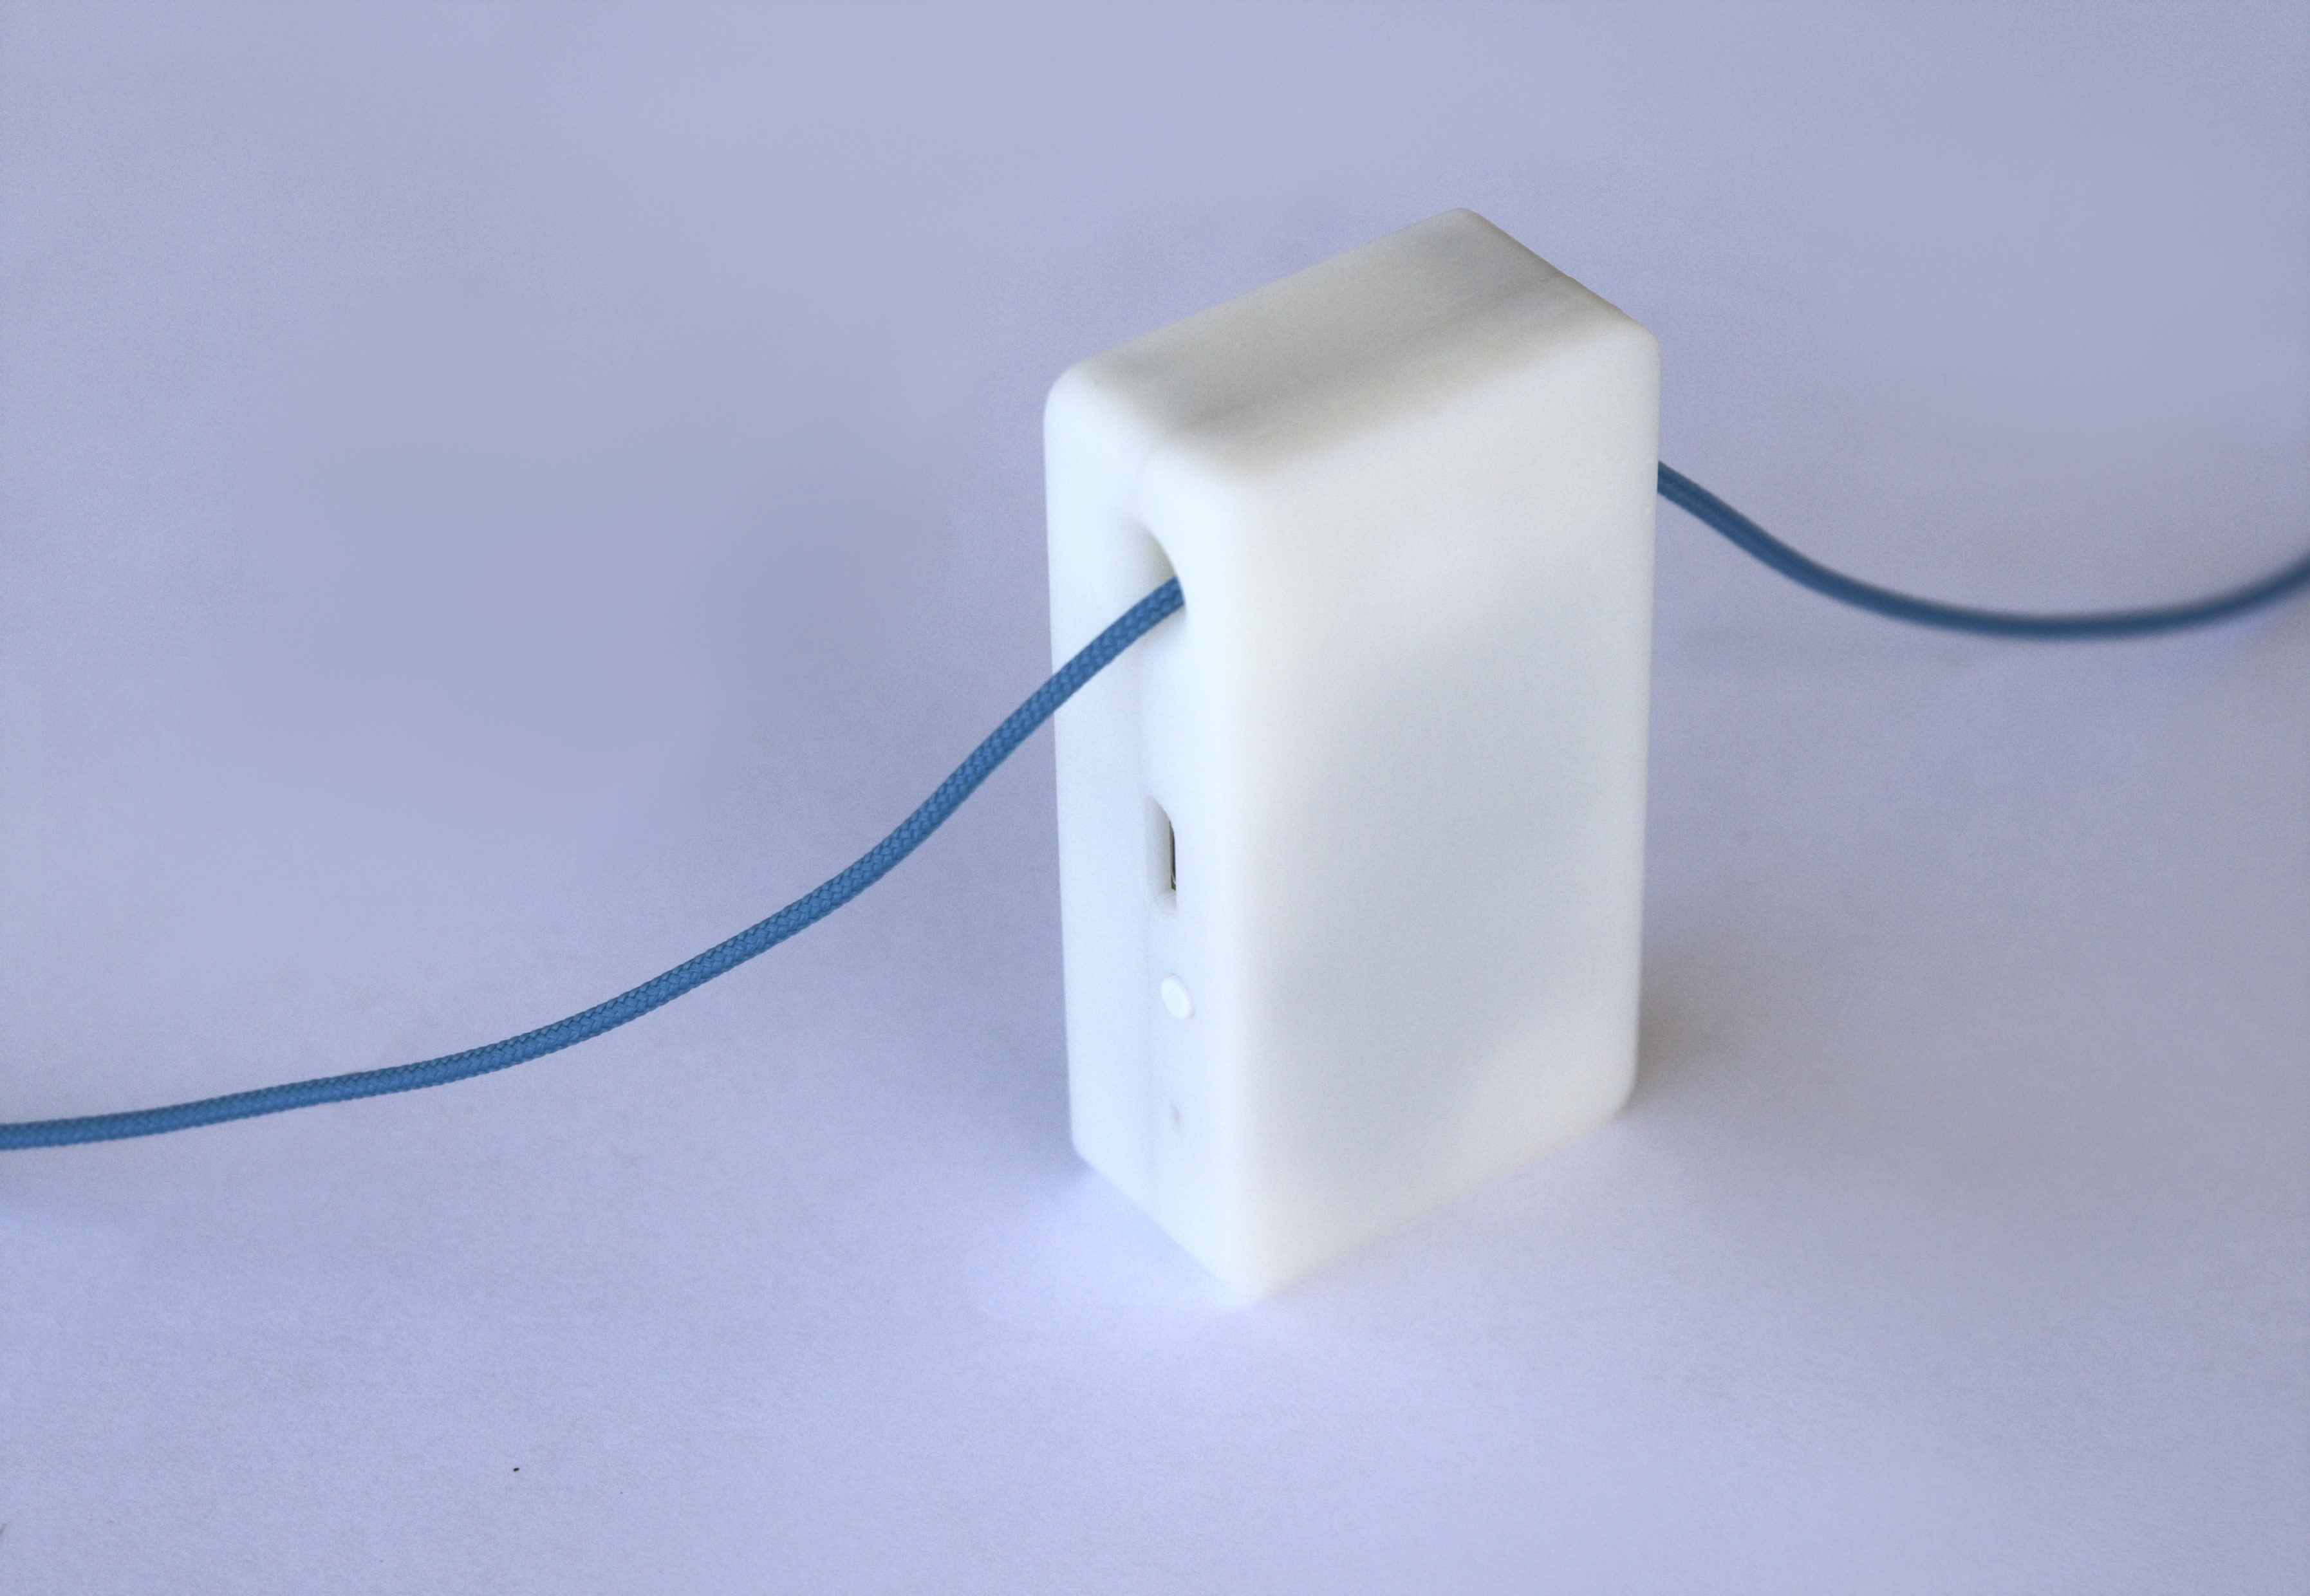
\includegraphics[width=8cm]{images/cutting-test}
	\caption{Cutting tests performed with the Reefing-System}
	\label{fig:cutting-test}
\end{figure}

\subsubsection{Scope of Test}
The scope of the cutting tests is to work out the cutting speed and repeatability. In particular, the following functions were tested:
\begin{itemize}
    \item Temperature of the ceramic heating element
    \item Time to cut reefing line 
    \item Variance in cutting time
\end{itemize}

\subsubsection{Acceptance criteria}
The test is successful if
\begin{itemize}
    \item The reefing line is always cut
    \item The time to cut, for the same setup, stays within a standard deviation of 5 seconds 
\end{itemize}

\subsection{Test Setup}
The Reefing System powered the heating element with a fully charged battery for both tests, and the heating element voltage was set to the maximum 12.2\,V. All tests were performed at an ambient temperature of 24\,$^\circ$C.

\subsubsection{Temperature measurement}
In order to generate a temperature curve of the heating element, a multimeter with a thermocouple was used. The thermocouple was firmly pressed against the surface of the heating element to get a reading close to the actual surface temperature. With a camera, the multimeter's display was recorded. The video was then used to get the data points. This test was repeated three times to get a better estimate. 

\subsubsection{Cutting Tests}
For the cutting tests, a paracord made out of nylon was used. The lines had a diameter of 1.4\,mm and 2.0\,mm. For testing the impact of force on the reefing line, a weight was added to one side of the paracord and suspended in air. The other end was tied down on a table. The time from the initiation of the cut to the separation was measured with a stopwatch. 

\subsection{Results}
\subsubsection{Temperature measurement}
A temperature curve was plotted using Python and matplotlib. The temperature increase is quite linear initially but drops off towards the end of the 30-second testing duration. As seen in Figure \ref{fig:temperature}, the experiment was repeated three times, and the corresponding temperature curves are relatively similar. A maximum temperature of 360\,$^\circ$C can be expected after 30 seconds.

\begin{figure}[h!]
	\centering
	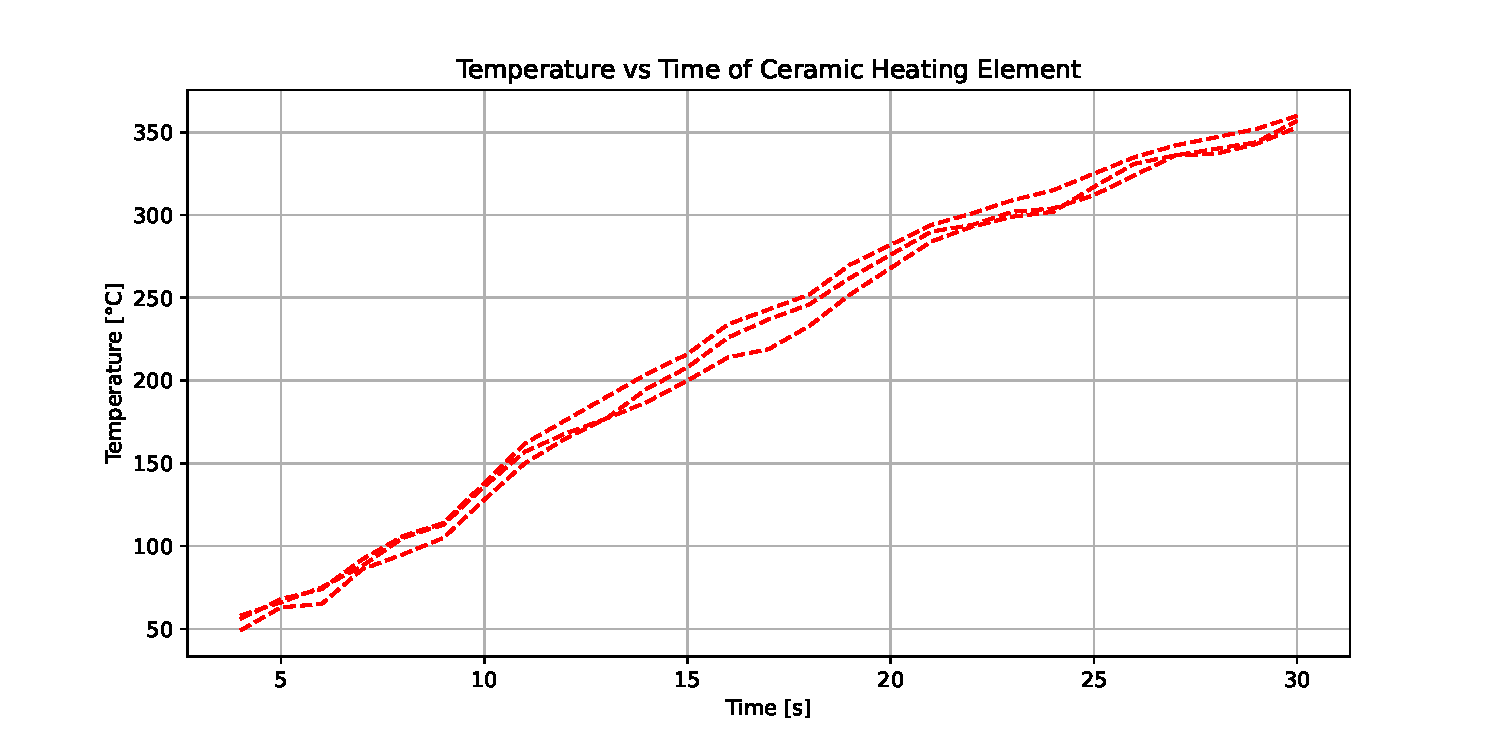
\includegraphics[width=\textwidth]{plots/temperature}
	\caption{Temperature plot of ceramic heating element}
	\label{fig:temperature}
\end{figure}

\subsubsection{Cutting Tests}
Four series of cutting tests were performed. For each series, six tests were performed to get a valid standard deviation. From the tests performed, it can be concluded that the standard deviation is a lot smaller than initially expected. Even when taking into account all measurements from both lines and forces, the standard deviation is still bellow 1.5\,s. 

\begin{table}[h]
    \centering
    \begin{tabular}{ m{4cm} | m{1.5cm} | m{1.5cm} } 
      \hline
      Force                 & \multicolumn{1}{c}{0.098\,N} & \multicolumn{1}{|c}{9.8\,N}  \\ \hline
      Time Delay            & \multicolumn{1}{c}{22.2}    & \multicolumn{1}{|c}{20.8}       \\
                            & \multicolumn{1}{c}{22.6}    & \multicolumn{1}{|c}{21.4}       \\
                            & \multicolumn{1}{c}{23.6}    & \multicolumn{1}{|c}{20.9}       \\
                            & \multicolumn{1}{c}{23.0}    & \multicolumn{1}{|c}{21.4}       \\
                            & \multicolumn{1}{c}{23.5}    & \multicolumn{1}{|c}{20.8}       \\
                            & \multicolumn{1}{c}{23.3}    & \multicolumn{1}{|c}{20.4}       \\
                            & \multicolumn{1}{c}{}        &  \multicolumn{1}{|c}{}          \\
      Mean                  & \multicolumn{1}{c}{23.06}   &\multicolumn{1}{|c}{20.95}      \\
                            & \multicolumn{1}{c}{}        &  \multicolumn{1}{|c}{}          \\
      Standard Deviation    & \multicolumn{1}{c}{0.572}   &\multicolumn{1}{|c}{0.482}      \\
    \end{tabular}
    \caption{\label{tab:nylon-2}Cutting tests performed with a 2.0\,mm nylon line}
\end{table}

\begin{table}[h]
    \centering
    \begin{tabular}{ m{4cm} | m{1.5cm} | m{1.5cm} } 
      \hline
      Force                 & \multicolumn{1}{c}{0.098\,N} & \multicolumn{1}{|c}{9.8\,N}  \\ \hline
      Time Delay            & \multicolumn{1}{c}{20.2}    & \multicolumn{1}{|c}{18.7}       \\
                            & \multicolumn{1}{c}{21.6}    & \multicolumn{1}{|c}{18.5}       \\
                            & \multicolumn{1}{c}{19.4}    & \multicolumn{1}{|c}{19.6}       \\
                            & \multicolumn{1}{c}{20.8}    & \multicolumn{1}{|c}{18.9}       \\
                            & \multicolumn{1}{c}{20.9}    & \multicolumn{1}{|c}{19.1}       \\
                            & \multicolumn{1}{c}{21.4}    & \multicolumn{1}{|c}{20.0}       \\
                            & \multicolumn{1}{c}{}        &  \multicolumn{1}{|c}{}          \\
      Mean                  & \multicolumn{1}{c}{20.70}   &\multicolumn{1}{|c}{19.13}      \\
                            & \multicolumn{1}{c}{}        &  \multicolumn{1}{|c}{}          \\
      Standard Deviation    & \multicolumn{1}{c}{0.811}   &\multicolumn{1}{|c}{0.568}      \\
    \end{tabular}
    \caption{\label{tab:nylon-14}Cutting tests performed with a 1.4\,mm nylon line}
\end{table}

\subsubsection{Test success}
The cutting and heating tests confirmed the system's reliability and exceeded the required standard deviation substantially. These numbers should not be taken as facts, as conditions during flight could impact performance. For example, airflow and line movement can increase the time to separation.

\newpage

\section{Simulation}
Before implementing the state estimation on the hardware, a simulation was written in Python to validate the performance.

\subsubsection{Scope of Test}
The simulation is used to validate the state estimation model and to tune the gains of the Kalman filter. In detail, the following functions should be tested:
\begin{itemize}
    \item Correctness of Kalman filter model
    \item Test finite state machine 
    \item Correctness of deployment altitude
\end{itemize}

\subsubsection{Acceptance criteria}
The test is successful if
\begin{itemize}
    \item The altitude and velocity estimation is accurate
    \item The Kalman filter can be tuned to acceptable levels
    \item The finite state machine working as expected
    \item The estimated cutting point is within 50\,m of the targeted altitude
\end{itemize}

\subsection{Test Setup}
For the test, the entire state estimation algorithm and the finite state machine were implemented in Python. Data from previous rocket flights are used for the simulation. Different flight profiles can be passed through to determine the system's effectiveness. The main altitude was set to 100 meters above ground level, and the burn duration is estimated to be 10 seconds.


In order to compare the estimations, raw data and moving averages are displayed in the same plot. The derivative of a moving average was taken for the velocity estimation since raw data had way too much noise.

The data used for the simulations were collected from previous rocket flights from ARIS using the same barometer. Therefore the noise and accuracy closely match the expected data from the Reefing System. Furthermore, the data is collected at 100\,Hz, which also matches the sampling speed on the Reefing System.  

\newpage

\subsection{Results}

\subsubsection{Kalman filter tuning}\label{filter-tuning}
Two parameters of the Kalman filter are used to tune the dynamics of the filter. The gain $R$, the altitude measurement covariance $\sigma_R$ and $Q$, the acceleration covariance $\sigma_a$. 

By analyzing previous flight data and the datasheet from the barometer, a measurement covariance of 5\,m was chosen. The acceleration covariance was experimentally selected by running a series of simulations. As shown in Figure \ref{fig:tune-velocity} it can be observed that the lower the covariance is, the smoother or less responsive the velocity estimation becomes. A smooth velocity estimation is beneficial for the application as it improves the deployment estimate. Thus a value of 5\,{m/s}$^2$ was selected. While the velocity is more irregular than lower $Q$ values, the altitude estimate, as seen in Figure \ref{fig:tune-altitude}, is closer to the real world.   

\begin{figure}[h!]
	\centering
	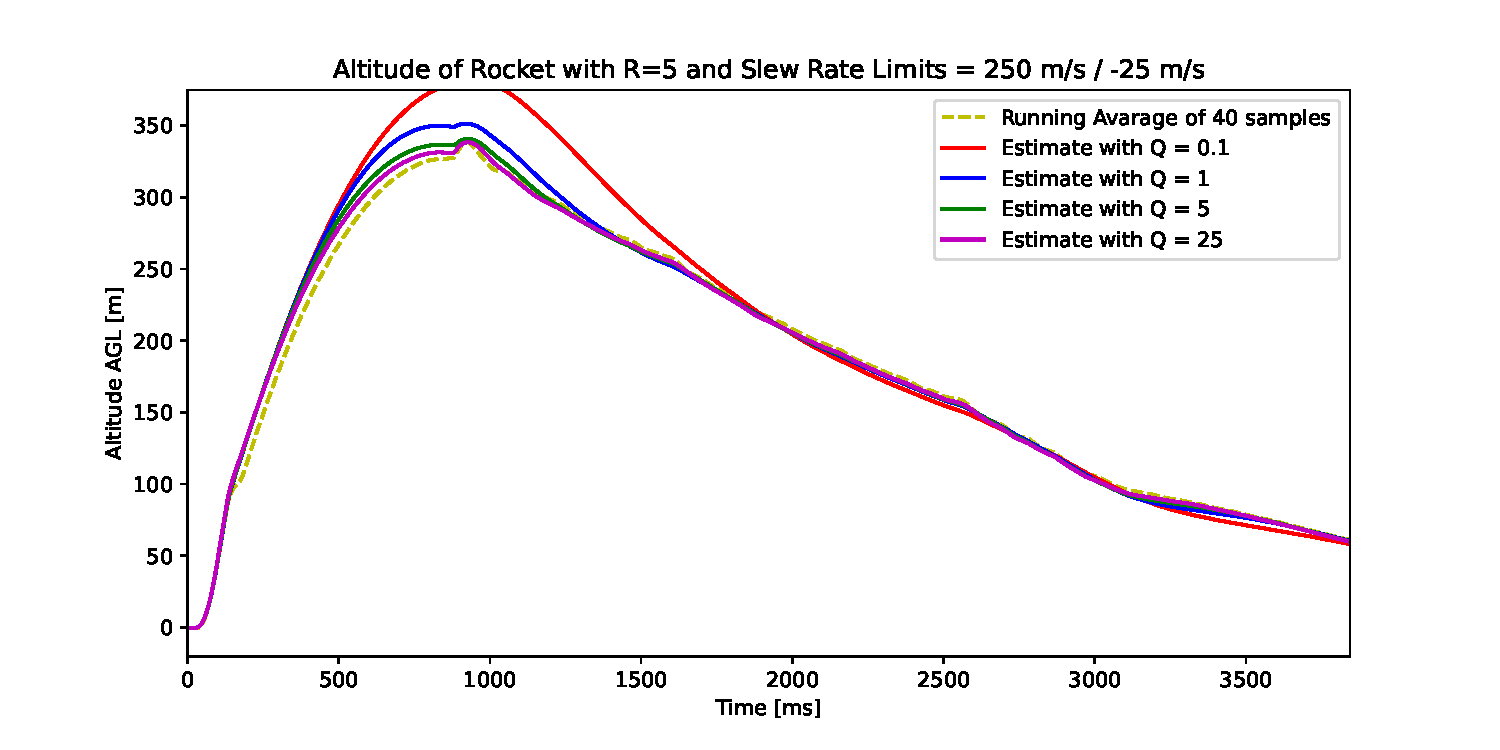
\includegraphics[width=\textwidth]{plots/altitude-tune}
	\caption{Altitude plot of flight simulation}
	\label{fig:tune-altitude}
\end{figure}

\begin{figure}[h!]
	\centering
	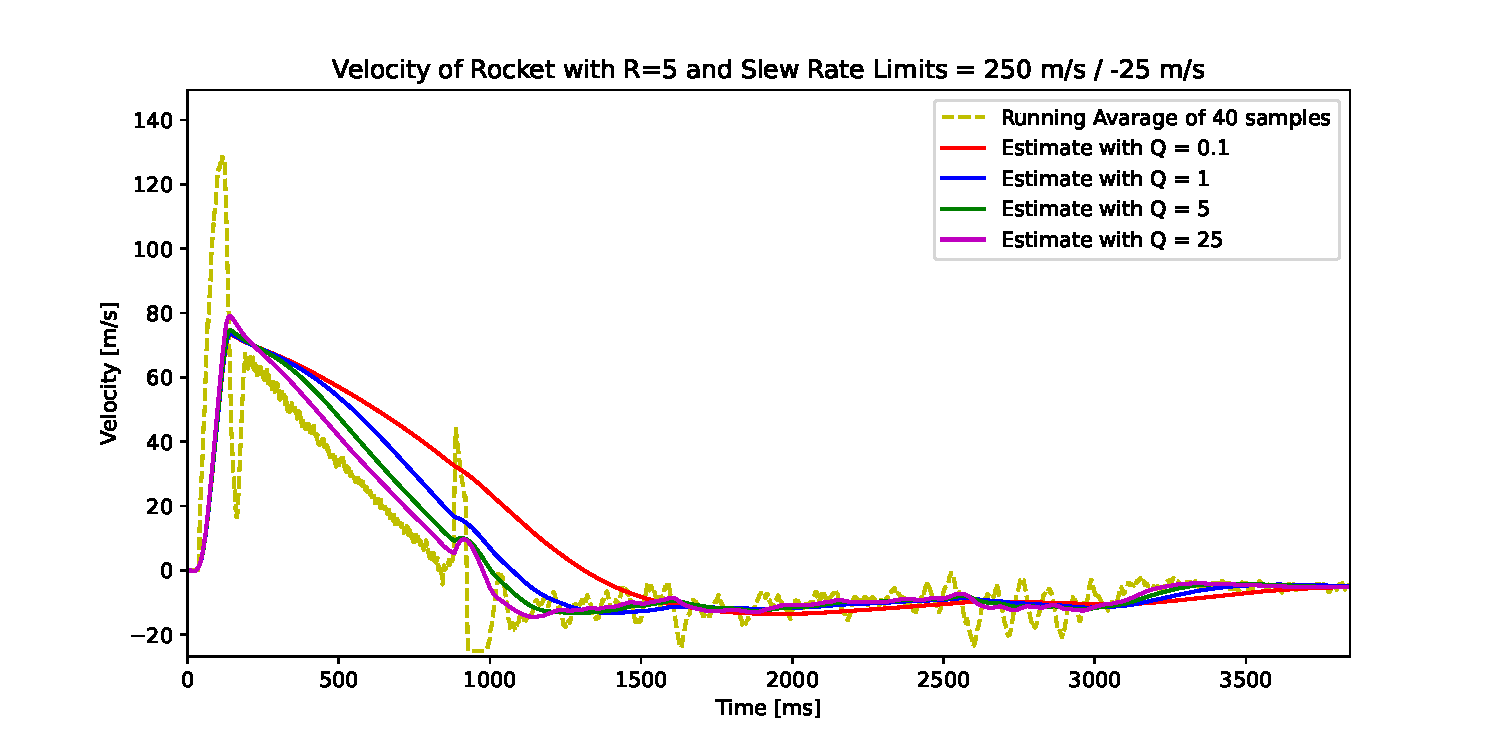
\includegraphics[width=\textwidth]{plots/velocity-tune}
	\caption{Velocity plot of flight simulation}
	\label{fig:tune-velocity}
\end{figure}

\subsubsection{Test success}
The state estimation is working as expected, and especially the velocity estimation is significantly improved over the running average as shown in Figure \ref{fig:sim-velocity}. The state estimation and the finite state machine make it possible to accurately predict the flight phases and the point where the heating element gets turned on. The estimated cutting point matches the requested altitude closely. The simulation made it possible to find an appropriate filter tune, and the Kalman filter matches the model. 

\begin{figure}[h!]
	\centering
	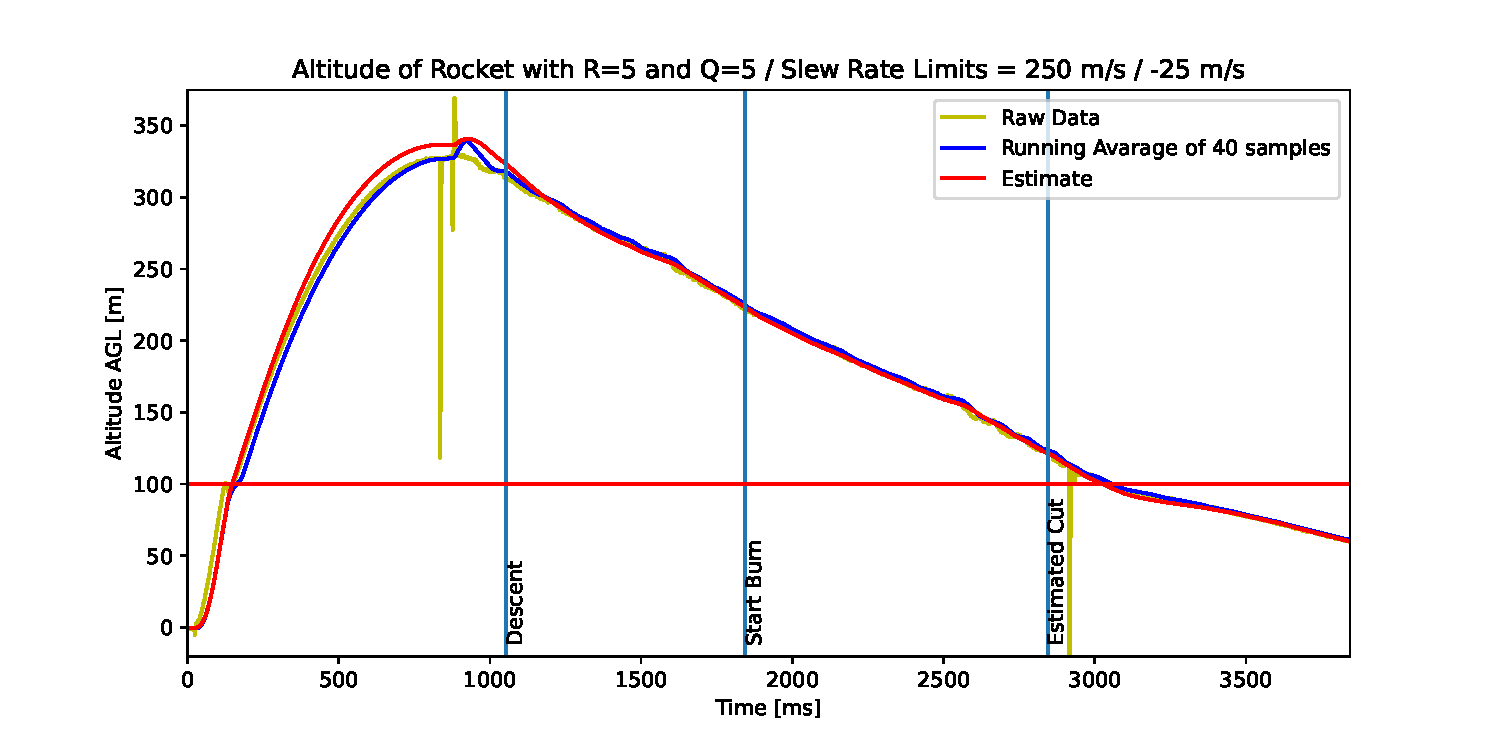
\includegraphics[width=\textwidth]{plots/sim-altitude}
	\caption{Altitude plot of flight simulation}
	\label{fig:sim-altitude}
\end{figure}

\begin{figure}[h!]
	\centering
	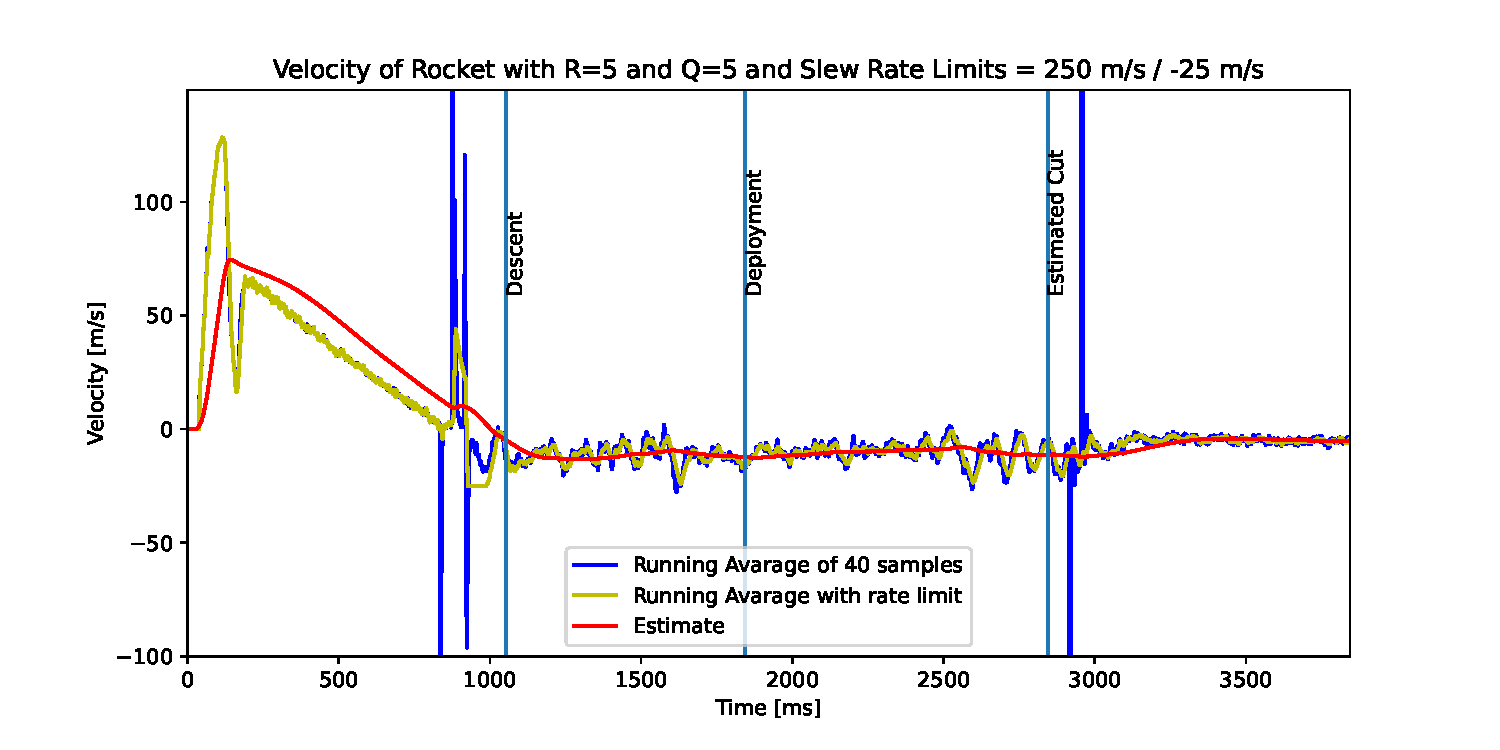
\includegraphics[width=\textwidth]{plots/sim-velocity}
	\caption{Velocity plot of flight simulation}
	\label{fig:sim-velocity}
\end{figure}

\newpage

\section{Firmware Validation}
To validate that all tasks are executed on time and that no stack overflow occurs, the \acrshort{rtos} was traced.

\begin{figure}[h!]
    \centering
	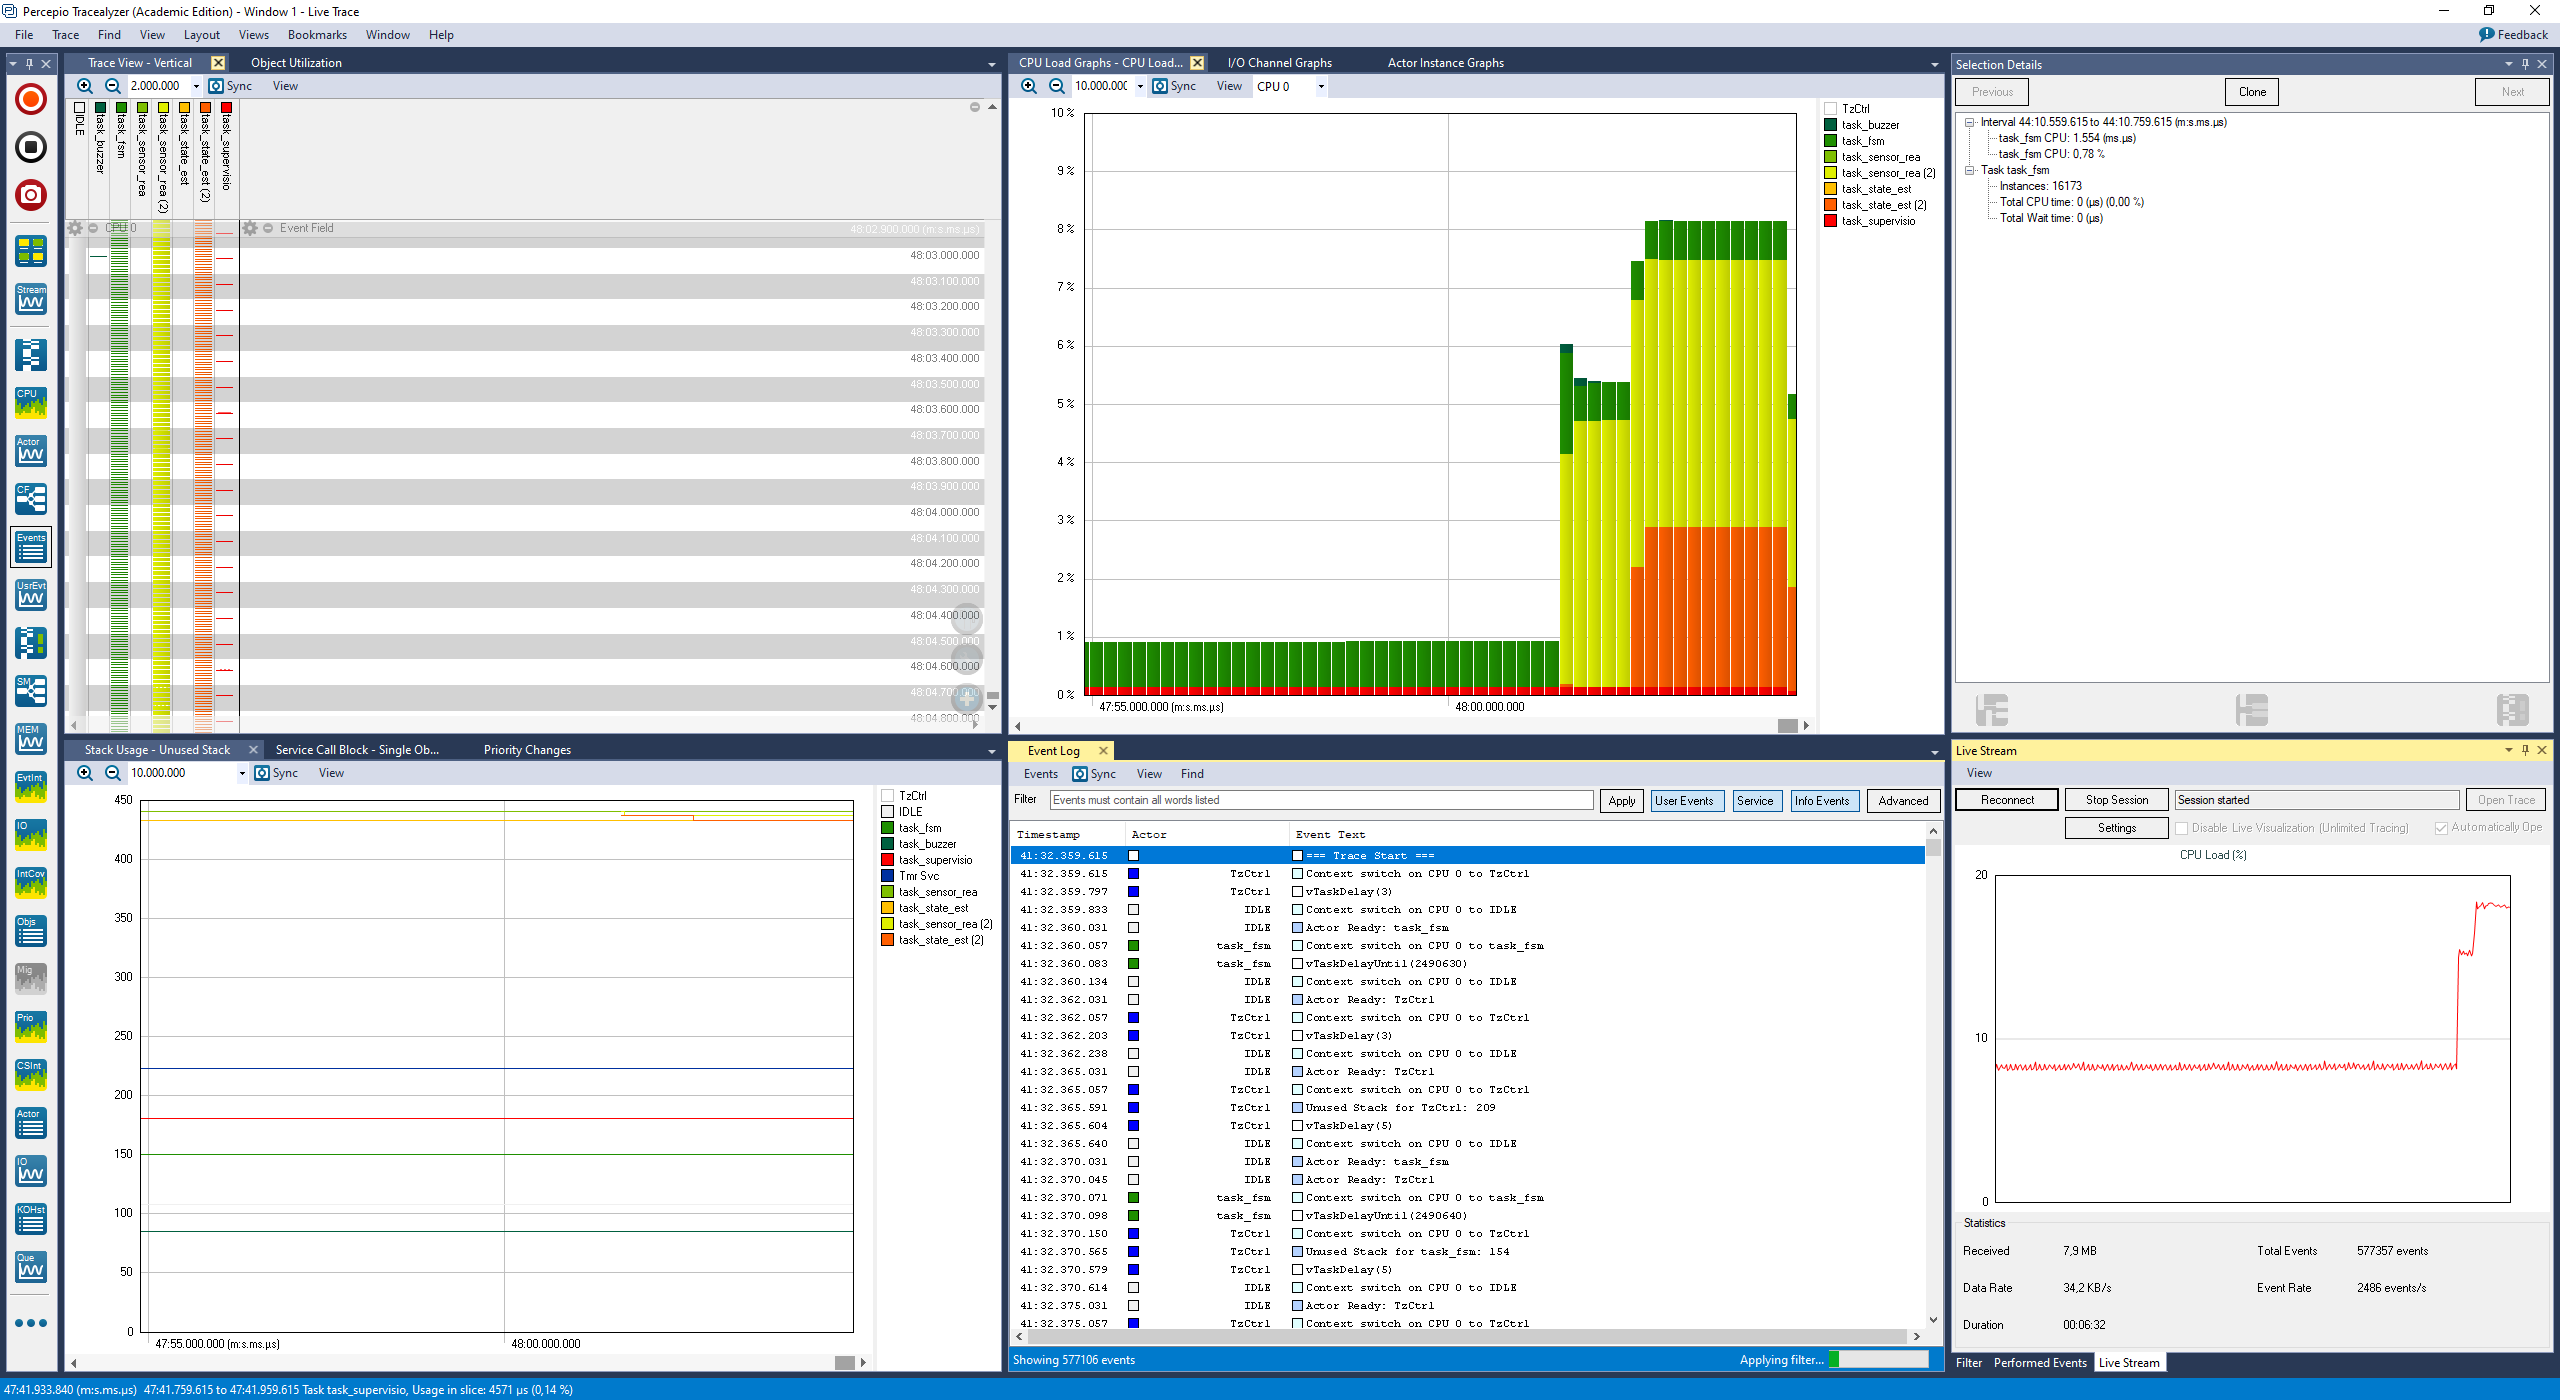
\includegraphics[width=10cm]{images/tracealyzer}
	\caption{Overview of trace views in Tracealyzer 4}
	\label{fig:tracealyzer}
\end{figure}

\subsubsection{Scope of Test}
The scope of the firmware validation is to verify the operation during all phases of flight. In detail, the following functions should be tested:
\begin{itemize}
    \item Task execution timings
    \item \acrshort{cpu} utilization
    \item Task stack usage
    \item Dynamic task starting and stopping
\end{itemize}

\subsubsection{Acceptance criteria}
The test is successful if
\begin{itemize}
    \item All task execution timings are as expected
    \item The \acrshort{cpu} usage stays bellow 75\,\%
    \item All tasks have at least 64 integers free stack
    \item Dynamic starting and stopping of the tasks works without any issues
\end{itemize}

\subsection{Test Setup}
Tracealyzer is a solution for visual trace diagnostics, giving embedded software developers insight into the runtime world. This tool allows for easier debugging of system-level issues and helps improve the software's design and performance. For the validation, a framework was added to the firmware to print out trace data over the \acrshort{usb} port. Percepio, the developer of Tracealyzer, provides the framework. While the trace is enabled, the \acrshort{cli} is disabled to not generate package collisions over the \acrshort{usb}.

\subsection{Results}
\subsubsection{Measurements and Observations}
From the \acrshort{cpu} load graph, it is easily recognizable that there is more than enough headroom for additional processing. During the flight, the maximum reached \acrshort{cpu} usage does not exceed 9\,\%. As shown in Figure \ref{fig:cpu-usage} the two tasks that require the most time to execute are the state estimation and sensor read task. This behavior is expected, as the sensor readout is done with all blocking functions and is therefore bound to \acrshort{spi} speeds. The state estimation requires the second-longest time to execute. The execution time for the state estimation is mainly the processing time for all the filters. The buzzer task is not fixed to a sampling frequency. Therefore it only utilizes \acrshort{cpu} time whenever the buzzer is beeping. The time it takes to print out the trace information is contained in the TzCtrl generated by the Tracealyzer framework and is not enabled in the trace.  

\begin{figure}[h!]
    \centering
	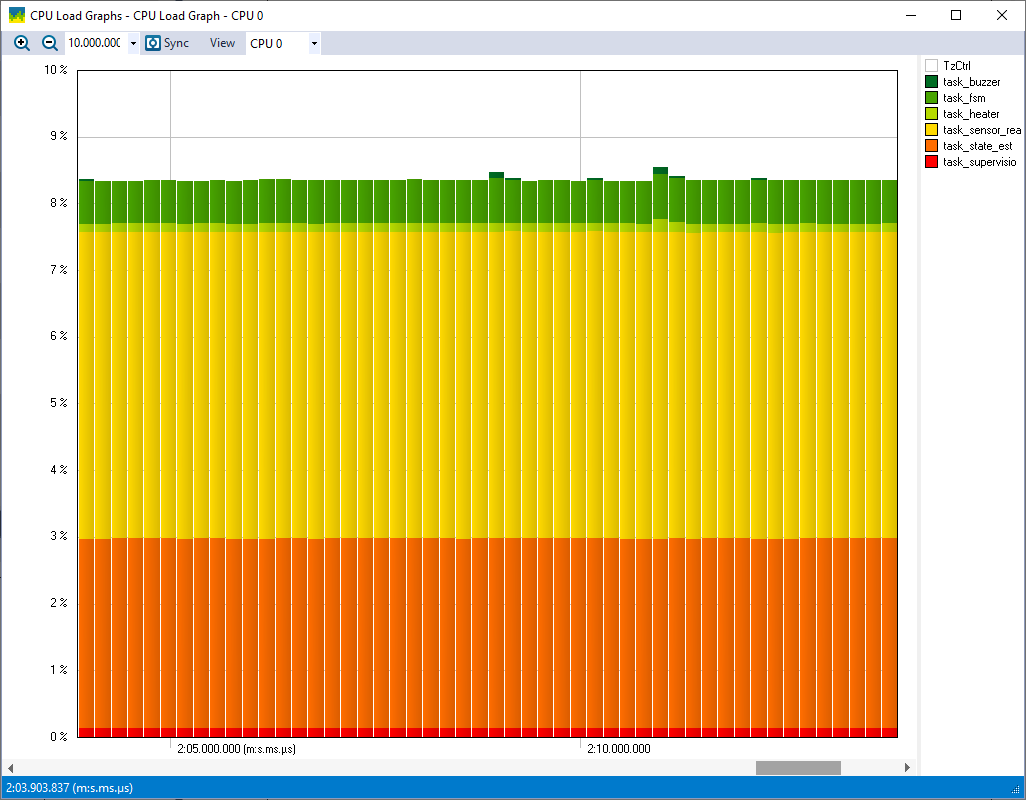
\includegraphics[width=7.8cm]{images/cpu-usage}
	\caption{CPU usage during flight with all tasks running}
	\label{fig:cpu-usage}
\end{figure}

The dynamically starting and stopping of the tasks were tested by switching the device from the idle mode to the ready mode and back. As soon as the state is changed, all required tasks are started, as shown in Figure \ref{fig:cpu-start}. The state estimation does not execute immediately after it is started, allowing for all the sensors to be initialized and read out at least once.

\begin{figure}[h!]
    \centering
	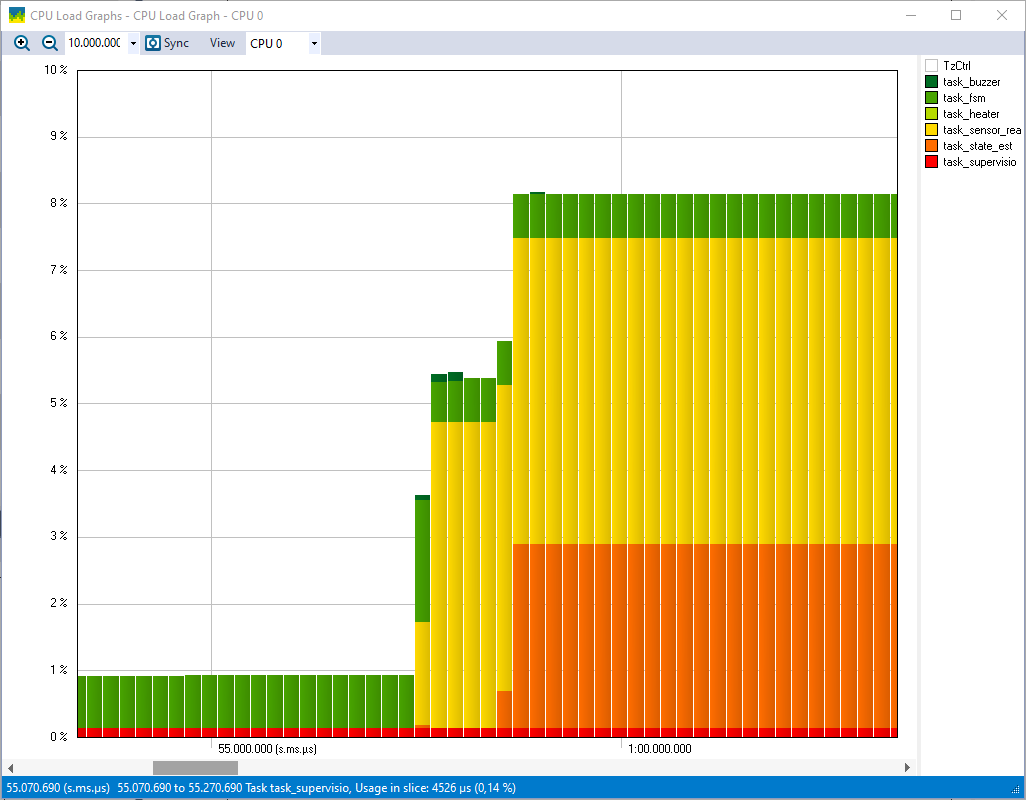
\includegraphics[width=7.8cm]{images/cpu-start}
	\caption{Dynamic starting of tasks in runtime}
	\label{fig:cpu-start}
\end{figure}

The timings were further validated by looking at the flow chart of task execution, depicted in Figure \ref{fig:cpu-flow}. Almost all time is spent just waiting for tasks to be ready for execution. The state estimation and the \acrshort{fsm} task are executed with a frequency of 100\,Hz while the sensor read task executes twice as often to read out the temperature and pressure.
\begin{figure}[h!]
    \centering
	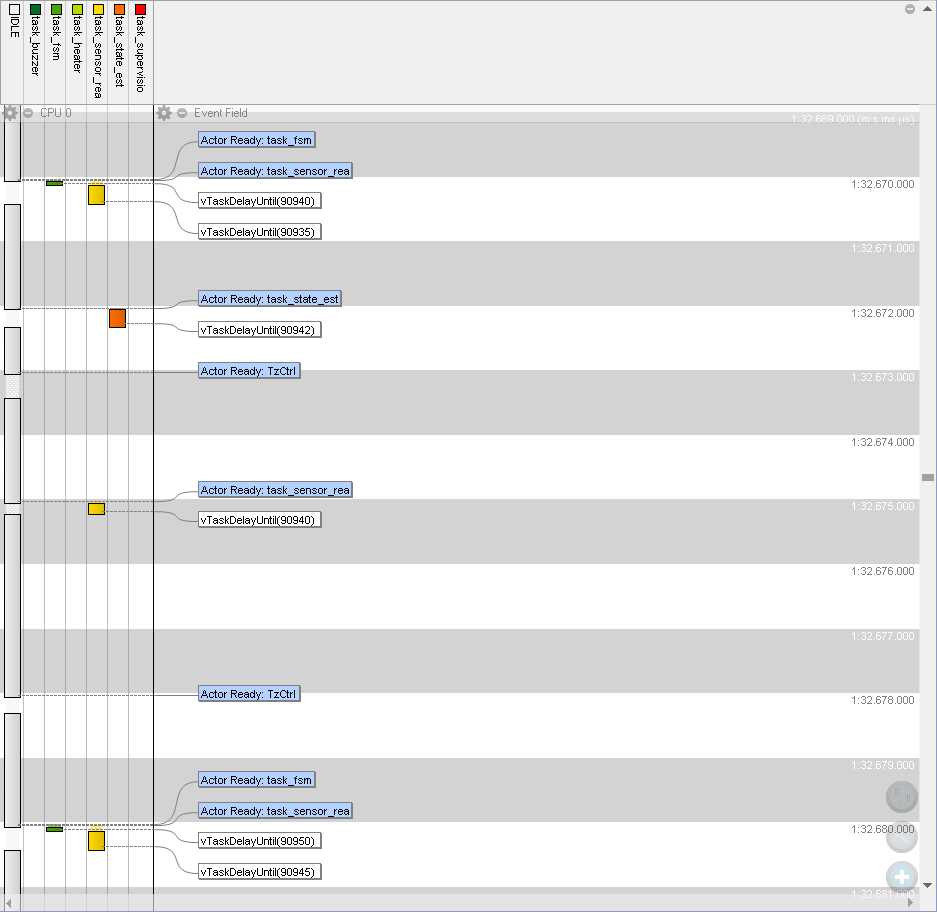
\includegraphics[width=7.8cm]{images/cpu-flow}
	\caption{Trace view of task execution}
	\label{fig:cpu-flow}
\end{figure}

Last but not least, the stack usage of all tasks was readout. The stack usage in FreeRTOS is not defined in bytes but in 32-bit integers. All tasks have more than 64 integers of stack left.


\subsubsection{Test success}
With the help of Tracealyzer, it was possible to prove that all timings and the stack usage are within an acceptable range. Furthermore, during testing, no unexpected observations were discovered.

The only part of the software that could not be analyzed with the trace is the \acrshort{cli}. Since both the trace and \acrshort{cli} share the \acrshort{usb} port, the task is disabled while tracing. Luckily this is not an issue for flight, as the \acrshort{cli} task is not running during that phase.

\newpage

\section{Drone Flight}
The purpose of the drone flight is to validate the state estimation before flying on a rocket. The test took place on the 12th of May, 2022. 

\begin{figure}[h!]
	\centering
	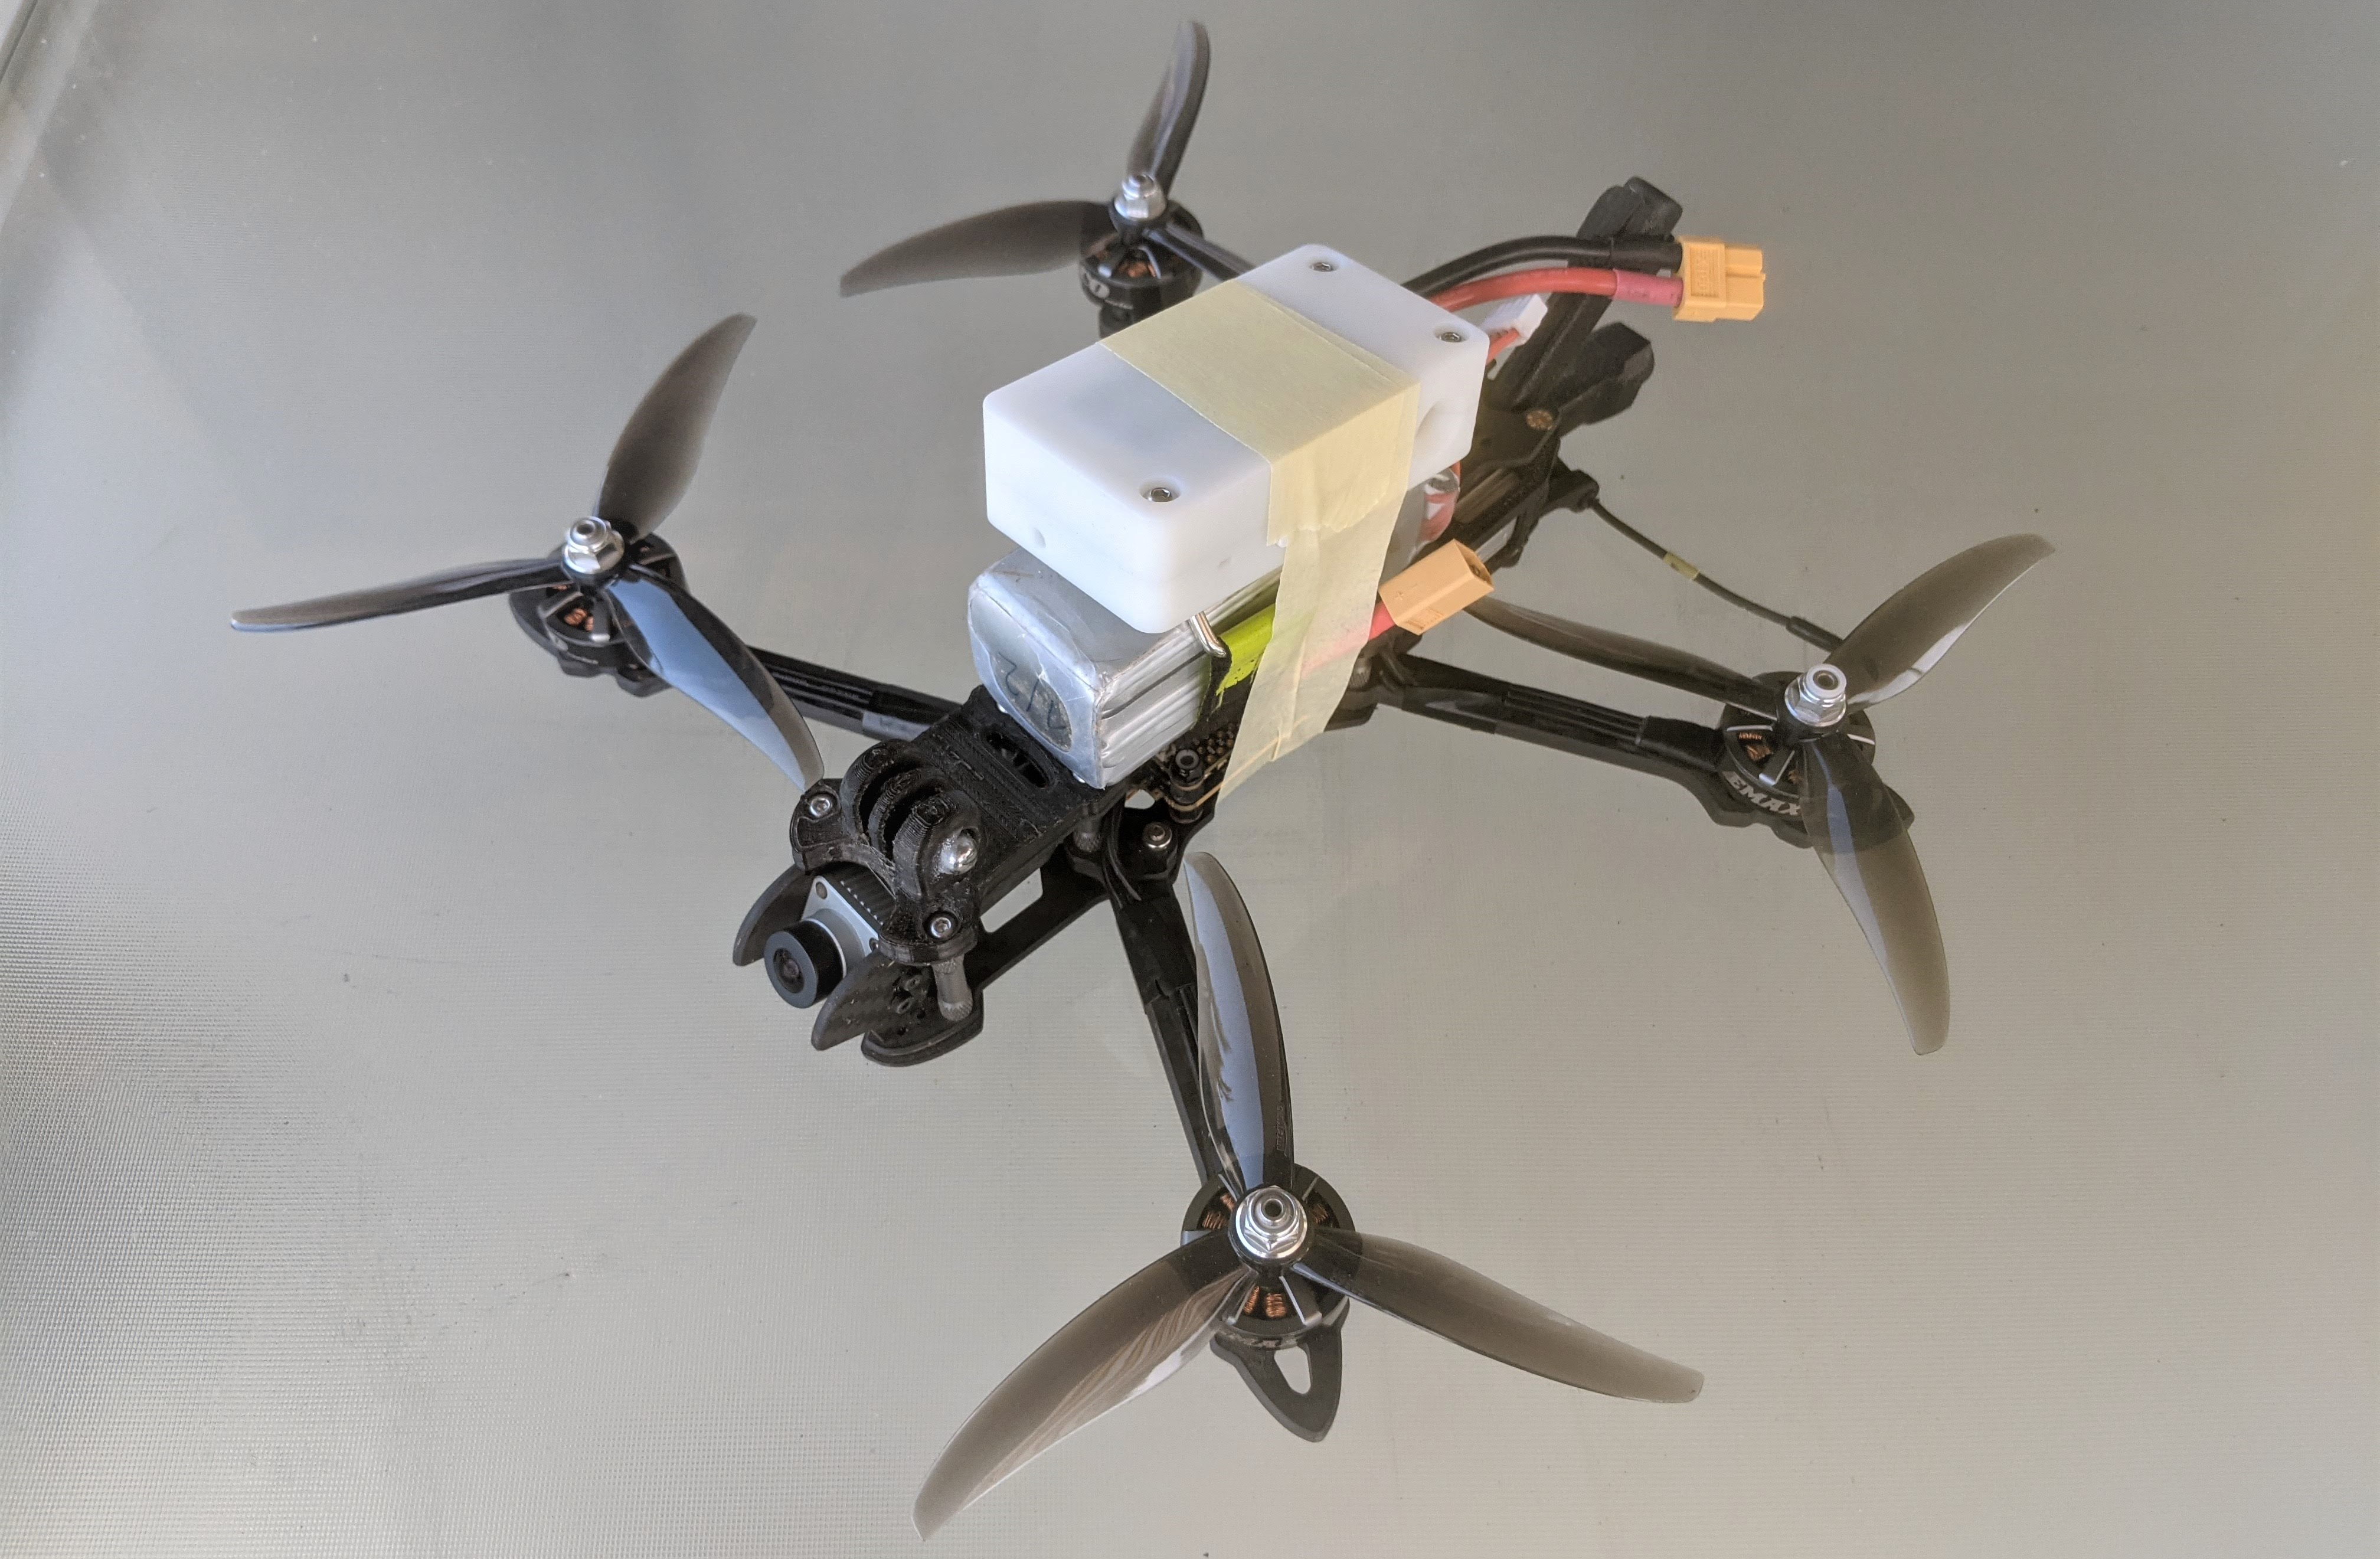
\includegraphics[width=\textwidth]{images/fpv}
	\caption{\acrshort{fpv} drone used for test flight with reefing system taped on top}
	\label{fig:fpv-drone}
\end{figure}

\subsubsection{Scope of Test}
The scope of the drone flight is to validate the state estimation. In detail, the following functions should be tested:
\begin{itemize}
    \item Liftoff detection with accelerometer
    \item Kalman Filter velocity and altitude estimation
    \item Correct state switching
    \item Data logging
\end{itemize}

\subsubsection{Acceptance criteria}
The test is successful if
\begin{itemize}
    \item All flight phases are detected
    \item The Kalman Filter estimations are realistic
    \item The data can be retrieved and analyzed after the test
\end{itemize}

\subsection{Test Setup}
The drone used for the test is a \acrshort{fpv} racing drone, built for high-speed maneuvers. With accelerations of up to 4\,g, the drone allows the simulation of a rocket flight. During this test, no reefing line was inserted to avoid stings from getting entangled in the propellers. For that reason, the burn duration was set to 5 seconds, and the main altitude was left at the default 100\,m.

In order to reproduce the flight profile of a rocket as closely as possible, the drone accelerates upward as fast as possible. At around 150\,m above ground level, the power is reduced for it to descend back to the ground.

\subsection{Results}
\subsubsection{Measurements and Observations}
The full duration of the drone flight was logged to the onboard memory. The flight logs were parsed and plotted using the jupyter notebook. The generated plots are shown in Figure \ref{fig:drone-altitude} and \ref{fig:drone-velocity}. 

\begin{figure}[h!]
	\centering
	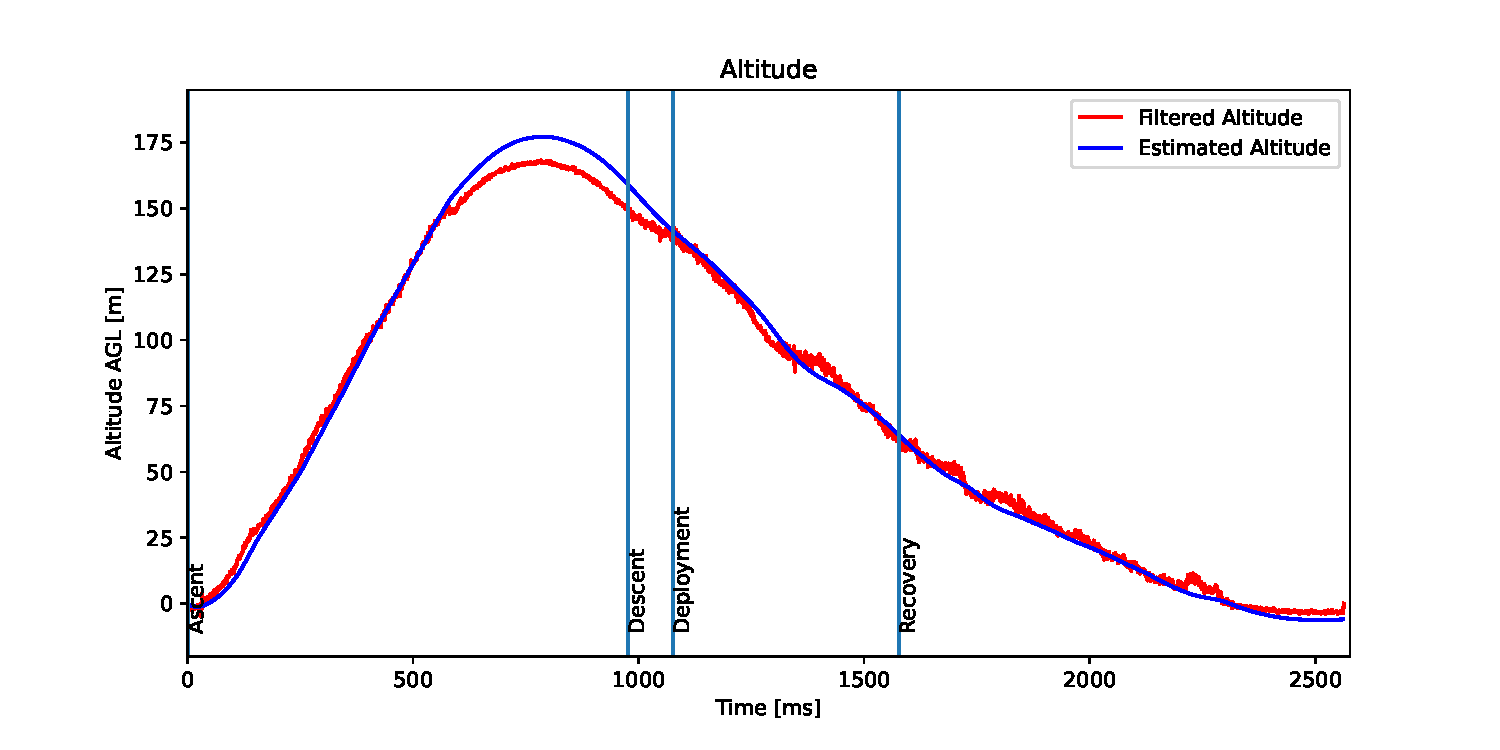
\includegraphics[width=\textwidth]{plots/drone-altitude}
	\caption{Altitude plot from flight log}
	\label{fig:drone-altitude}
\end{figure}

\begin{figure}[h!]
	\centering
	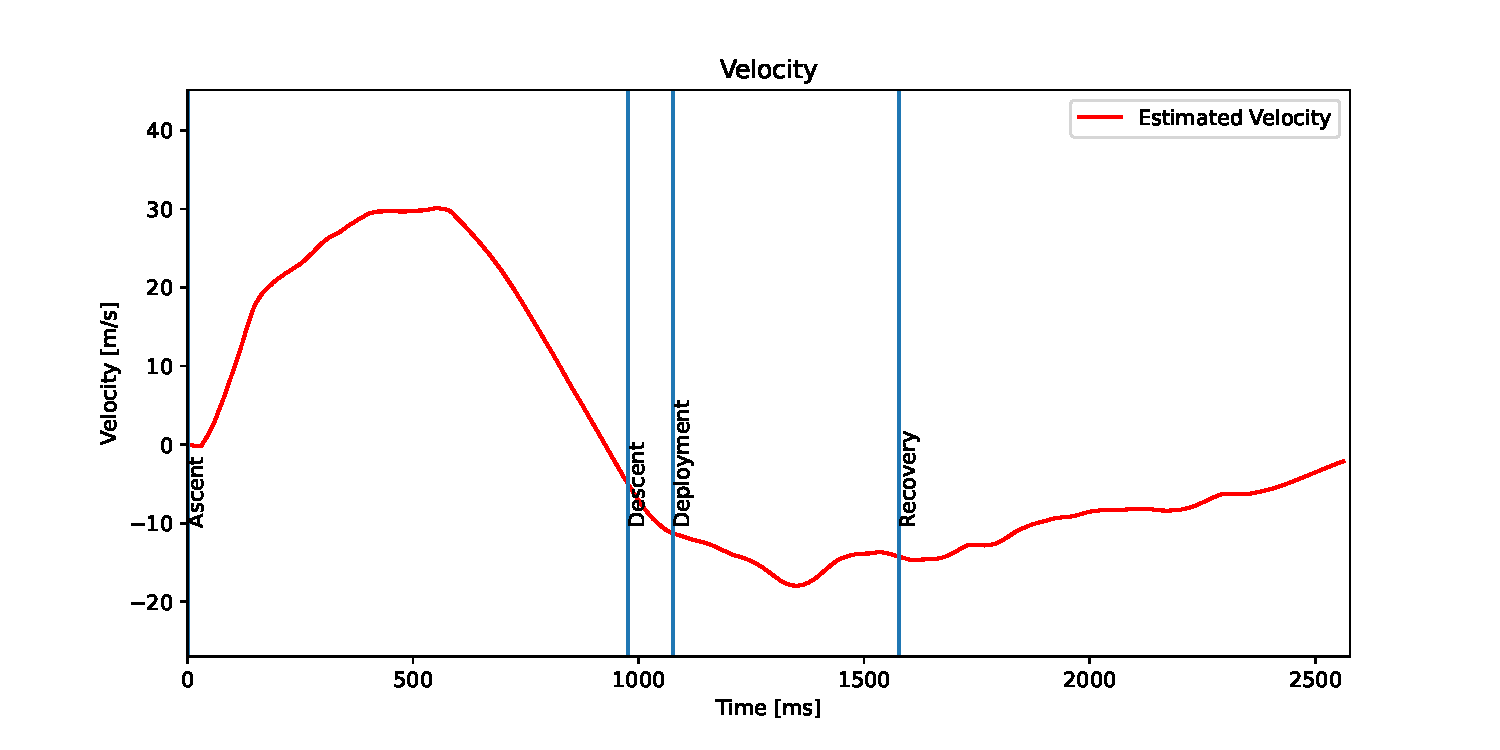
\includegraphics[width=\textwidth]{plots/drone-velocity}
	\caption{Velocity plot from flight log}
	\label{fig:drone-velocity}
\end{figure}

The filtered altitude is the moving average altitude calculated before passing it into the Kalman filter. The estimated altitude is a lot smoother than the filtered altitude. 

The filter dynamics are tuned for a rocket flight, where velocity changes are slowly reaching zero. Therefore the filter overestimated the apogee and consequently detected the descent phase late. Since the drone flight is very short, this delay is visible. However, it is of no concern, as rocket flights are a lot longer.

The velocity estimate is lagging about two seconds behind the actual velocity. As already explained in Section \ref{filter-tuning} the filter is purposely tuned to be slow but accurate. For that reason, the result is expected.

\subsubsection{Test success}
Overall, the test was successful and provided data about the state estimation performance in flight. Compared to simulations done beforehand, the actual data matches them perfectly. No unexpected observations were discovered, and the system is ready for the first rocket flight. 


\newpage

\section{Rocket Flight}
In order to fully validate the system, a full-scale rocket flight was conducted on the 14th of May, 2022. The rocket flight was in cooperation with ARGOS, a Swiss rocketry association. 

\begin{figure}[h!]
	\centering
	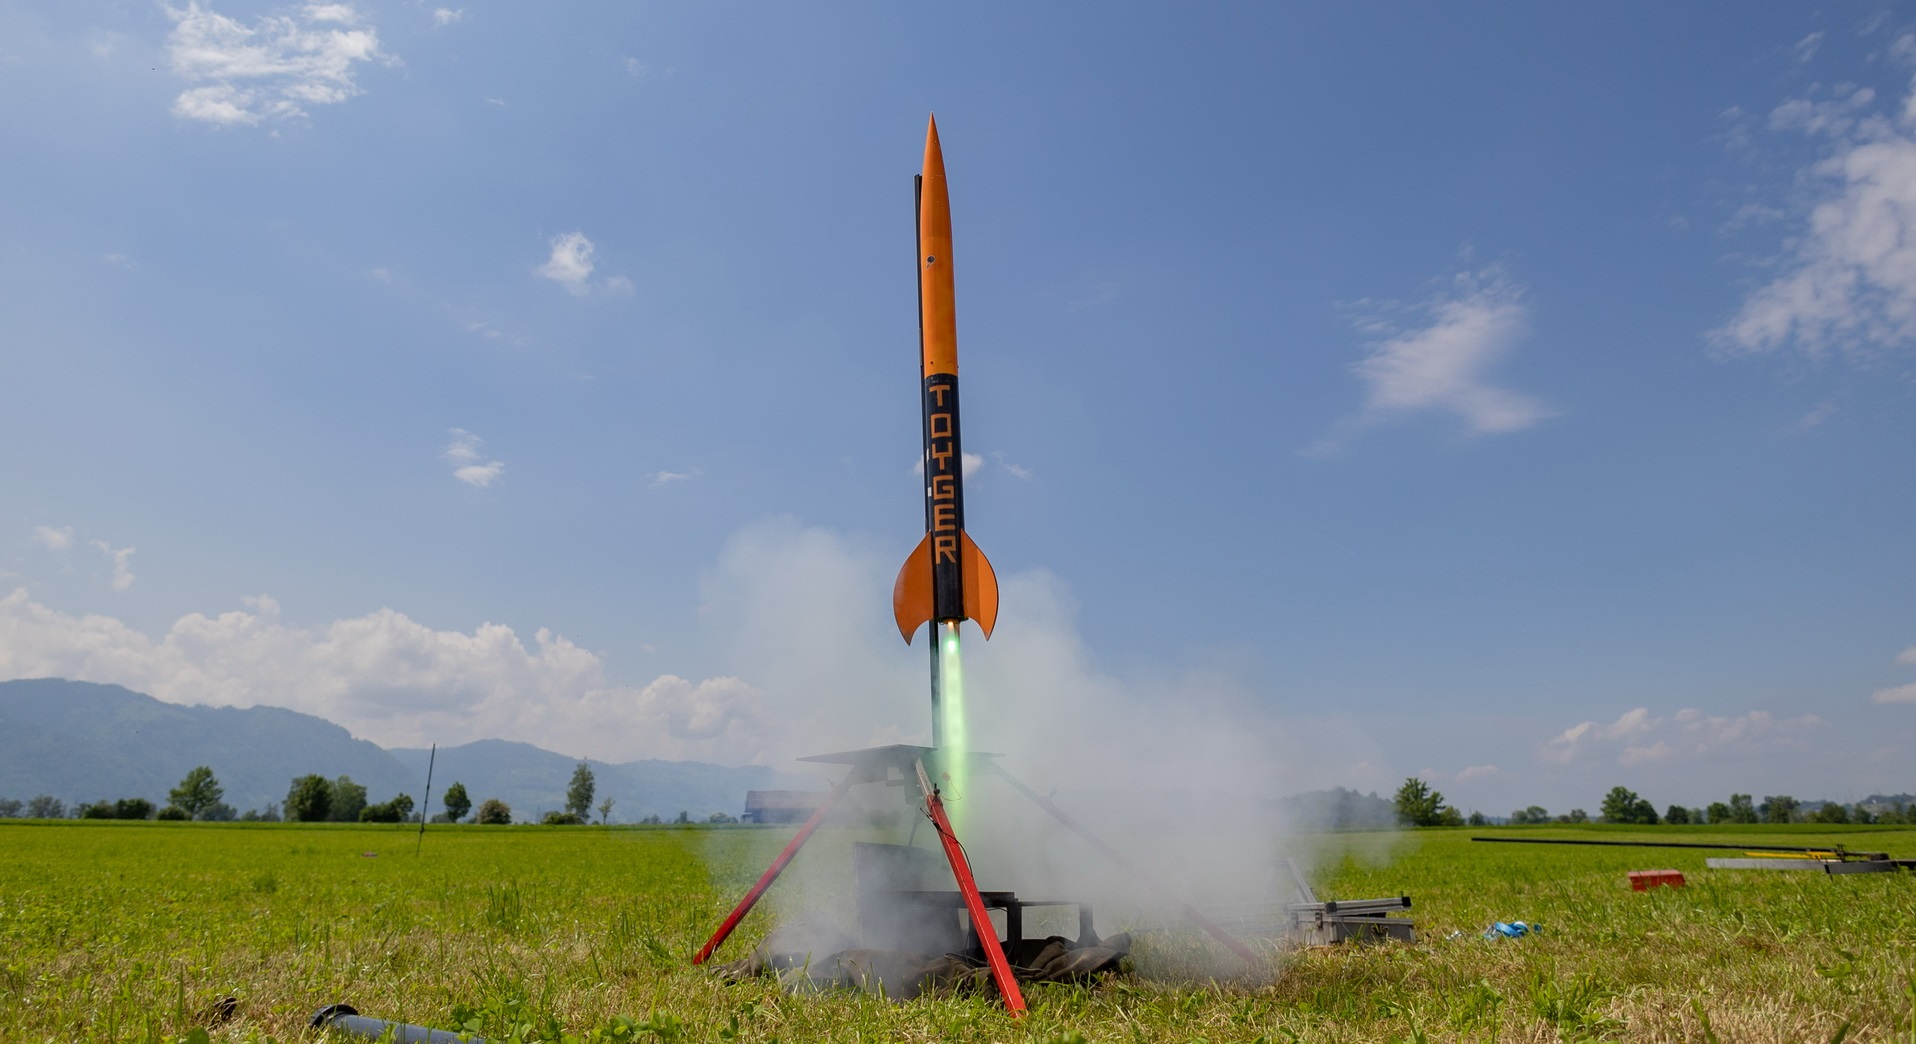
\includegraphics[width=\textwidth]{images/toyger}
	\caption{Rocket \emph{Toyger} lifting off from the launch rail in Kaltbrunn}
	\label{fig:operation}
\end{figure}

\subsubsection{Scope of Test}
The scope of the rocket flight test is to verify the operation in a real-world environment. In detail, the following functions should be tested:

\begin{itemize}
    \item Power management over an extended period
    \item Liftoff detection while the reefing computer is in sleep mode (wake up from accelerometer)
    \item Kalman Filter velocity and altitude estimation
    \item Separation of the reefing line
    \item Data logging during the flight
\end{itemize}

\subsubsection{Acceptance criteria}
The test is successful if
\begin{itemize}
    \item The reefing line gets separated during the descent of the rocket
    \item The Kalman Filter roughly estimates the altitude and velocity of the rocket
    \item The data can be retrieved and analyzed after the test
\end{itemize}

\subsection{Test Setup}
The rocket named Toyger is the rocket conducting the test. It is 178cm long and has a dry mass of almost 2kg. The rocket was constructed from a build kit and is made out of cardboard and wood. Epoxy was added to the outer walls to strengthen the material.

The rocket has flown five times before and is an excellent fit for the test as it is a proven design. 
\subsubsection{Parachute Setup}
The rocket is equipped with a single 137cm diameter parachute for recovery. A reefing ring was added to each suspension line of the parachute, and a reefing line was pulled through. In addition, the Reefing System was added to the line and securely mounted to the upper side of a canopy gore using tape. 

The parachute gets ejected at apogee by a redundant black powder charge, pushing the motor section tube and nosecone apart. The parachute is pulled out, and the descent of the flight starts. 

\subsubsection{Reefing System Configuration}
The biggest concern before the test was that the heating element does not reach the appropriate temperature in time to separate the reefing line. Because of that, the following configuration was chosen.

Preheating of the heating element is turned on from the rocket's launch. A burn duration of 30\,s was configured, forcing the computer to start heating at full power beginning at apogee. 

\subsection{Results}

\subsubsection{Measurements and Observations}
During the flight, the system was constantly logging data. After the flight, the logs were pulled from the device and plotted. The plots are shown in Figure \ref{fig:argos-altitude} and \ref{fig:argos-velocity}. 

\begin{figure}[h!]
	\centering
	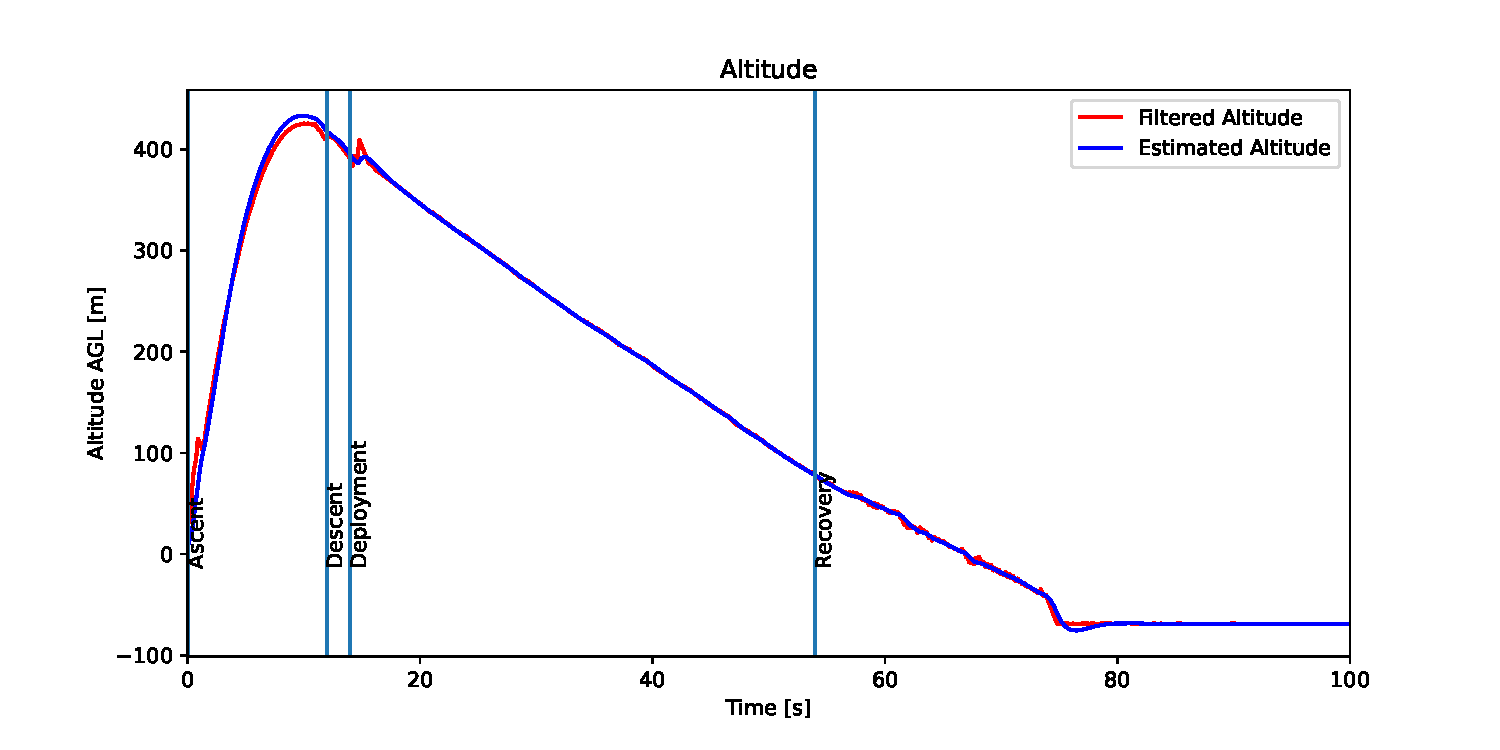
\includegraphics[width=\textwidth]{plots/argos-altitude}
	\caption{Altitude plot from flight log}
	\label{fig:argos-altitude}
\end{figure}

\begin{figure}[h!]
	\centering
	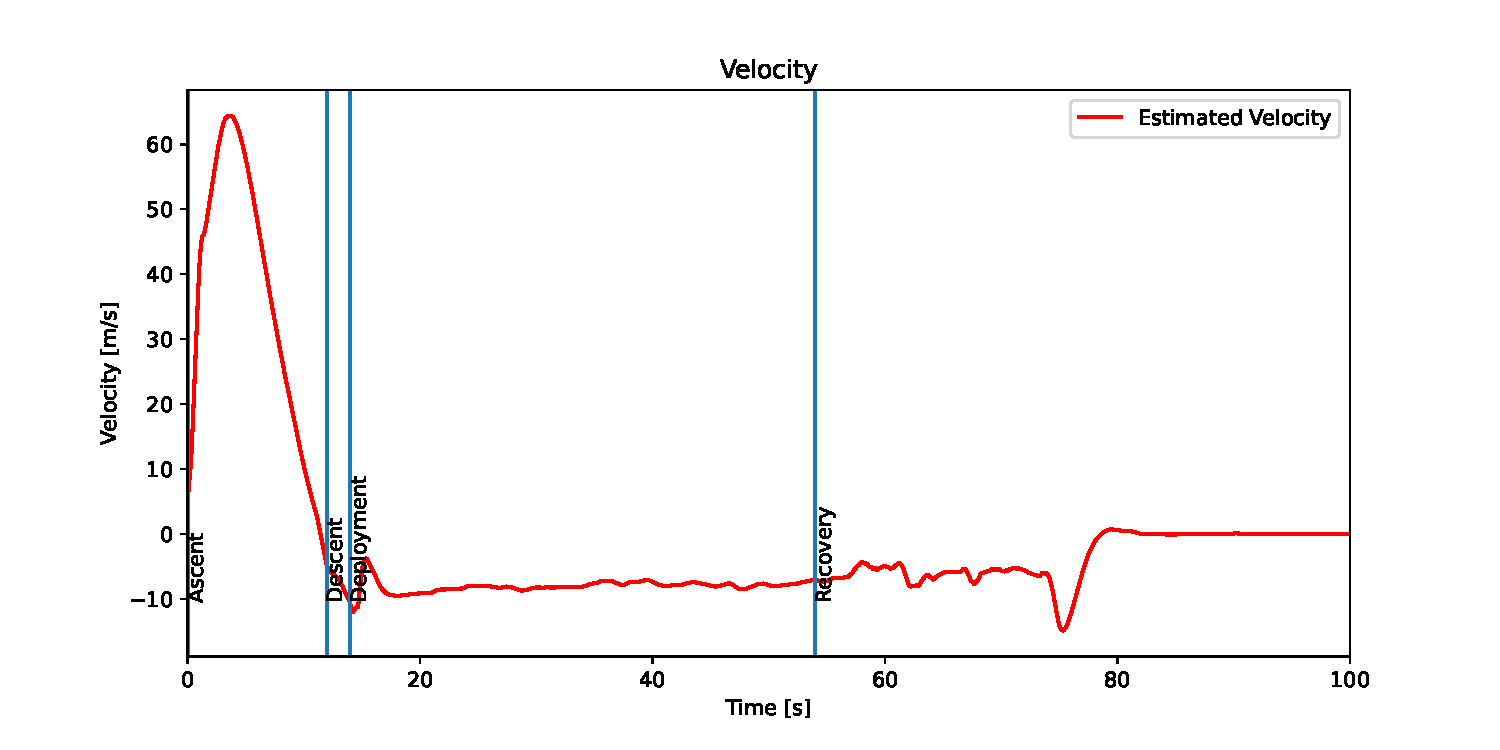
\includegraphics[width=\textwidth]{plots/argos-velocity}
	\caption{Velocity plot from flight log}
	\label{fig:argos-velocity}
\end{figure}

The state estimation worked flawlessly during all phases of the flight. One thing to note is that in Figure \ref{fig:argos-altitude} the estimated altitude did go below zero after touchdown, even though the rocket landed above its liftoff point. This occurrence can be explained by the fact that the system is sleeping before liftoff and does not adjust the zero altitude for about an hour. Temperature and pressure changes during that hour are not taken into account. This behavior was not unexpected but will need to be fixed in the future.  

After the rocket hit apogee, the parachute was ejected and immediately disreefed. Resulting in a slow descent to the ground. As shown in Figure \ref{fig:toyger-parachute} the reefing computer is still attached to the parachute, and the reefing line is cut.

\begin{figure}[h!]
	\centering
	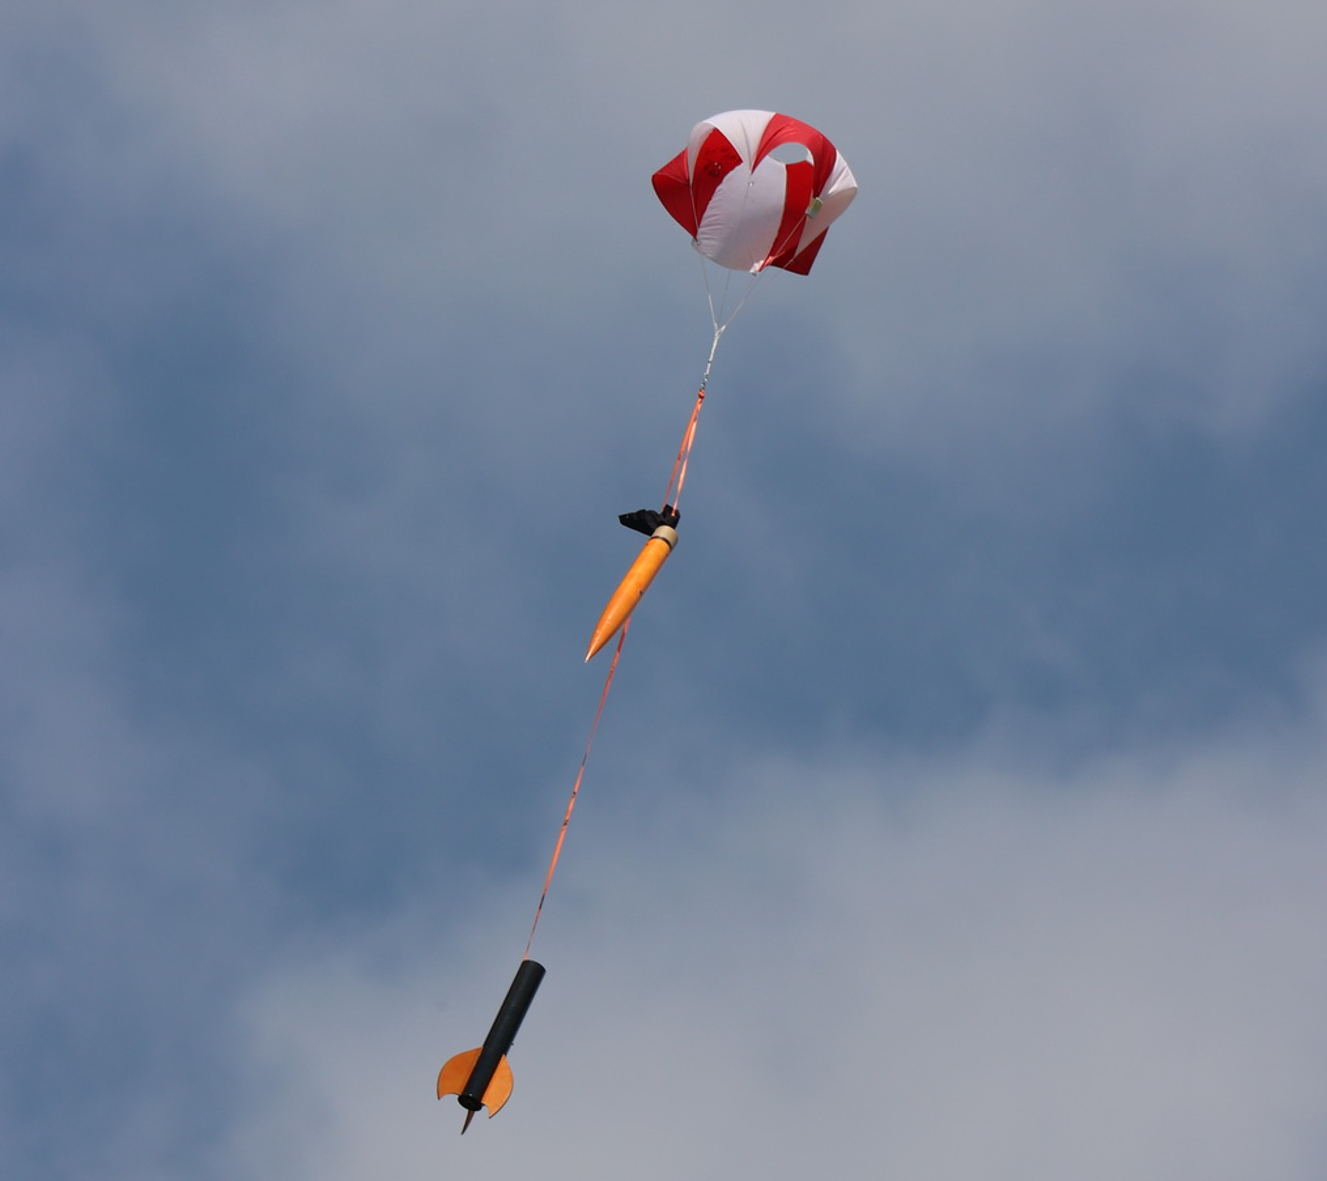
\includegraphics[width=10cm]{images/toyger-parachute}
	\caption{Descent with disreefed parachute}
	\label{fig:toyger-parachute}
\end{figure}

\subsubsection{Test success}
The reefing computer separated the line, logged all data during the flight, and estimated the velocity and altitude to acceptable levels. Therefore the test validated some of the most critical aspects of the flight. 

\subsubsection{Unexpected Observations}
One of the black powder charges failed to ignite at apogee, forcing the rocket into a free fall for around 6 seconds after apogee. Luckily the second black powder charge fired and ejected the parachutes. The cause is most likely improper preparation of the ejection mechanism and has nothing to do with the Reefing System.

On the other hand, a problem related to the Reefing System is the early separation of the reefing line. As soon as the parachute was ejected, the line separated, advancing it to the fully open stage. The behavior observed was not easily explainable in the beginning. Unfortunately, the line was not recovered after the flight as it was not attached to the parachute. Without the line, the conclusion is open to speculation. The line ripping from the shear forces was quickly disputed, as the shear strength of the reefing line is higher than the shear strength of the suspension line, therefore making it impossible for the reefing line to rip first. It was concluded that the temperature rise of the element was a lot quicker during the flight than during ground testing. The quicker temperature increase can be explained when taking into account external factors. The rocket was fully assembled and sitting in the sun for an hour, heating the inside to over 45$^{\circ}$C. During the rocket's ascent, the system was preheating the element for about 14 seconds. Without any air circulation and being well isolated by the parachute, the temperature most likely reached the melting point of the reefing line much quicker than in testing on an open bench. As a result, the line was melted enough to separate as soon as the parachute ejected.

Another observation after the flight is that the timestamp overflowed after 65.535 seconds. The cause of that is that a 16\,bit unsigned integer is used to timestamp the data. After 65535\,ms, the integer overflows and returns to zero. This issue will not be resolved on the computer side as the increase to a 32\,bit integer would reduce the number of data points significantly. The overflow does not impact data integrity and is only fixed in the parsing stage. Whenever the timestamp decreases, $2^{16}$ is added to the rest of the data points, fixing the issue altogether.

\subsubsection{Things to improve}
Although the test was overall very successful, there are some things to improve.
\begin{itemize}
    \item The ambient temperature needs to be considered when preheating the element. A software update that enables the preheating only while below a certain threshold can be easily added.
    \item More test flights are needed to improve the timing of the separation.
    \item The reefing line should always be attached to the parachute on the opposite side of the reefing cutter. The line can help a lot in the post-flight analysis. For example, burn marks on multiple spots of the line indicate that the line was moving a lot while the element was heating.
    \item Before liftoff, the system needs to periodically wake up and reset the liftoff position to prevent altitude drifts. 
\end{itemize}
